\begin{tikzpicture}[scale=\modDGHyperScale]
% dummy
\coordinate[overlay] (v-coord-0-0) at (1.5493, -0.052044) {};
\coordinate[overlay] (v-coord-1-0) at (-0.77925, 2.2516) {};
\coordinate[overlay] (v-coord-2-0) at (-1.0639, -2.5422) {};
\coordinate[overlay] (v-coord-3-0) at (2.0415, -0.66322) {};
\coordinate[overlay] (v-coord-5-0) at (-0.62401, 2.8627) {};
\coordinate[overlay] (v-coord-7-0) at (-0.40387, -1.4672) {};
\coordinate[overlay] (v-coord-9-0) at (-0.64703, 3.4923) {};
\coordinate[overlay] (v-coord-11-0) at (-0.095634, -0.24294) {};
\coordinate[overlay] (v-coord-13-0) at (0.3162, 0.94924) {};
\coordinate[overlay] (v-coord-15-0) at (1.0389, 1.9836) {};
\coordinate[overlay] (v-coord-17-0) at (-0.7275, 4.1156) {};
\coordinate[overlay] (v-coord-19-0) at (2.2842, -1.4097) {};

% id = 0, graphName = Graph 1
\node[modStyleDGHyperVertex, at=(v-coord-0-0)] (v-0-0) {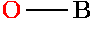
\includegraphics[scale=\modDGHyperImageScale] {out/000_g_0.1111110.pdf}\\{$\mathrm{Graph\ 1}$}};
% id = 1, graphName = Graph 2
\node[modStyleDGHyperVertex, at=(v-coord-1-0)] (v-1-0) {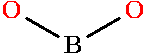
\includegraphics[scale=\modDGHyperImageScale] {out/001_g_1.1111110.pdf}\\{$\mathrm{Graph\ 2}$}};
% id = 2, graphName = Graph 3
\node[modStyleDGHyperVertex, at=(v-coord-2-0)] (v-2-0) {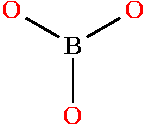
\includegraphics[scale=\modDGHyperImageScale] {out/002_g_2.1111110.pdf}\\{$\mathrm{Graph\ 3}$}};
% id = 3, graphName = p_{0,0}
\node[modStyleDGHyperVertex, at=(v-coord-3-0)] (v-3-0) {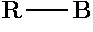
\includegraphics[scale=\modDGHyperImageScale] {out/004_g_3.1111110.pdf}\\{$\mathrm{p_{0,0}}$}};
% id = 5, graphName = p_{0,1}
\node[modStyleDGHyperVertex, at=(v-coord-5-0)] (v-5-0) {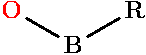
\includegraphics[scale=\modDGHyperImageScale] {out/005_g_4.1111110.pdf}\\{$\mathrm{p_{0,1}}$}};
% id = 7, graphName = p_{0,2}
\node[modStyleDGHyperVertex, at=(v-coord-7-0)] (v-7-0) {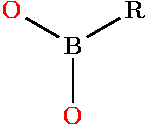
\includegraphics[scale=\modDGHyperImageScale] {out/006_g_6.1111110.pdf}\\{$\mathrm{p_{0,2}}$}};
% id = 9, graphName = p_{0,3}
\node[modStyleDGHyperVertex, at=(v-coord-9-0)] (v-9-0) {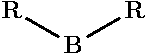
\includegraphics[scale=\modDGHyperImageScale] {out/007_g_9.1111110.pdf}\\{$\mathrm{p_{0,3}}$}};
% id = 11, graphName = p_{0,4}
\node[modStyleDGHyperVertex, at=(v-coord-11-0)] (v-11-0) {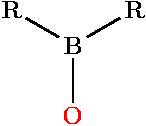
\includegraphics[scale=\modDGHyperImageScale] {out/008_g_10.1111110.pdf}\\{$\mathrm{p_{0,4}}$}};
% id = 13, graphName = p_{0,5}
\node[modStyleDGHyperVertex, at=(v-coord-13-0)] (v-13-0) {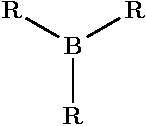
\includegraphics[scale=\modDGHyperImageScale] {out/009_g_12.1111110.pdf}\\{$\mathrm{p_{0,5}}$}};
% id = 15, graphName = p_{0,6}
\node[modStyleDGHyperVertex, at=(v-coord-15-0)] (v-15-0) {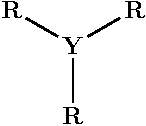
\includegraphics[scale=\modDGHyperImageScale] {out/010_g_13.1111110.pdf}\\{$\mathrm{p_{0,6}}$}};
% id = 17, graphName = p_{0,7}
\node[modStyleDGHyperVertex, at=(v-coord-17-0)] (v-17-0) {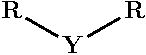
\includegraphics[scale=\modDGHyperImageScale] {out/011_g_14.1111110.pdf}\\{$\mathrm{p_{0,7}}$}};
% id = 19, graphName = p_{0,8}
\node[modStyleDGHyperVertex, at=(v-coord-19-0)] (v-19-0) {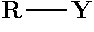
\includegraphics[scale=\modDGHyperImageScale] {out/012_g_15.1111110.pdf}\\{$\mathrm{p_{0,8}}$}};
% id = 4{ 'Graph 1' }, 'Mark', { 'p_{0,0}' }
\path[modStyleDGHyperConnector] (v-0-0) to node[auto, swap] {$\mathrm{r_{0}}$} (v-3-0);
% id = 6{ 'Graph 2' }, 'Mark', { 'p_{0,1}' }
\path[modStyleDGHyperConnector] (v-1-0) to node[auto, swap] {$\mathrm{r_{0}}$} (v-5-0);
% id = 8{ 'Graph 3' }, 'Mark', { 'p_{0,2}' }
\path[modStyleDGHyperConnector] (v-2-0) to node[auto, swap] {$\mathrm{r_{0}}$} (v-7-0);
% id = 10{ 'p_{0,1}' }, 'Mark', { 'p_{0,3}' }
\path[modStyleDGHyperConnector] (v-5-0) to node[auto, swap] {$\mathrm{r_{0}}$} (v-9-0);
% id = 12{ 'p_{0,2}' }, 'Mark', { 'p_{0,4}' }
\path[modStyleDGHyperConnector] (v-7-0) to node[auto, swap] {$\mathrm{r_{0}}$} (v-11-0);
% id = 14{ 'p_{0,4}' }, 'Mark', { 'p_{0,5}' }
\path[modStyleDGHyperConnector] (v-11-0) to node[auto, swap] {$\mathrm{r_{0}}$} (v-13-0);
% id = 16{ 'p_{0,5}' }, 'Unmark', { 'p_{0,6}' }
\path[modStyleDGHyperConnector] (v-13-0) to node[auto, swap] {$\mathrm{r_{1}}$} (v-15-0);
% id = 18{ 'p_{0,3}' }, 'Unmark', { 'p_{0,7}' }
\path[modStyleDGHyperConnector] (v-9-0) to node[auto, swap] {$\mathrm{r_{1}}$} (v-17-0);
% id = 20{ 'p_{0,0}' }, 'Unmark', { 'p_{0,8}' }
\path[modStyleDGHyperConnector] (v-3-0) to node[auto, swap] {$\mathrm{r_{1}}$} (v-19-0);
\end{tikzpicture}
